\documentclass[journal,10pt]{IEEEtran}
\usepackage{graphicx,booktabs,multirow,amsmath,amssymb,array,cite,url}
\graphicspath{{figures/}}
\hyphenation{dis-agree-ment inter-po-la-tion re-con-struc-tion}

\begin{document}
\title{Disagreement-Based Quality Assessment of MRI Slice Interpolation: Measurement Dependence and Anatomical Error}
\author{Anonymous Authors}
\markboth{IEEE Transactions on Medical Imaging, Manuscript Under Review}{}
\maketitle

\begin{abstract}
Agreement between deterministic MRI interpolators can hide substantial shared error. We study measurement dependence in 24 fastMRI brain examinations, 115 IXI brain examinations, and 22 NingXia knee series from eight patients, with additional analytical experiments on 125 TopCoW and 100 CAS2023 annotated angiograms. A complete 13-baseline, three-cohort benchmark contextualizes the study. Five neural architectures on both brain cohorts retain positive disjoint-minus-shared observable gains under exploratory simultaneous inference, while examination ranking is less robust. Raw-output reconstruction distinguishes prediction-derived bank masks from ground-truth support. In retrospective densification audits, all 26 fastMRI/NingXia Anchor-CV intervals cross zero after conditioning on current error. On IXI, normalizing both scores and benefit preserves positive association, whereas normalizing only one reverses ranking. Fixed linear/cubic estimators on TopCoW give local observable gains of 34.5 and 34.5 percentage points, but general-error ranking does not imply vessel-error ranking. A bright-anchor weighting rule motivated on TopCoW transfers without retuning to CAS2023: disjoint vessel-error correlations improve by .073 [.017,.130] and .070 [.014,.126] under two-pair simultaneous intervals. General-error ranking deteriorates, and vessel-risk coverage intervals cross zero. Shared-energy decompositions are algebraically coupled rather than independent mechanism tests. The results support anatomically specified quality assessment with explicit measurement, support, and scale contracts, without establishing calibrated uncertainty, diagnostic safety, or prospective acquisition utility.
\end{abstract}

\begin{IEEEkeywords}
Magnetic resonance imaging, slice interpolation, reliability, uncertainty, disagreement, measurement dependence.
\end{IEEEkeywords}

\section{Introduction}
\IEEEPARstart{A}{nisotropic} MRI volumes often have coarse through-plane resolution. Learned interpolation improves visual continuity and quantitative reconstruction \cite{peng2020saint,song2024i3net}, but a frozen deterministic model normally returns one image without stating when the missing anatomy is insufficiently constrained. A deployment-facing reliability signal must identify likely failure without accessing the unavailable dense target.

Ensembles, stochastic sampling, and test-time augmentation estimate uncertainty from output variation \cite{gal2016dropout,lakshminarayanan2017ensembles,edupuganti2021uncertainty,narnhofer2022bayesian}. Their premise is one-sided: disagreement witnesses a difference, while agreement need not imply correctness. Hu \emph{et al.} showed that variability-based uncertainty can miss systematic MRI reconstruction error \cite{hu2021predict}, and MRI ensembles have been evaluated under domain shift \cite{kuestner2024ensembles}. We investigate a complementary, physically auditable source of dependence: two interpolation contexts may reuse the same acquired slices and therefore inherit aligned errors that cancel in their difference.

Figure~\ref{fig:concept} summarizes the paired-reconstruction framework and the acquired-support MRA scoring branch. We reconstruct the same missing physical plane under contexts that either share no acquired anchors or maximally reuse them. The study does not claim a new correlated-error identity, a new reconstruction backbone, or calibrated uncertainty. Its contribution is a three-cohort medical-imaging characterization of how known measurement dependence changes error observability.

Our contributions include an acquired-only anatomical score with fixed-rule external MRA transfer, alongside: (i) a target-preserving neural measurement-dependence contrast across three cohorts and a frozen five-architecture replication on two independent brain cohorts; (ii) complete shared/observable error distributions, seven endpoints, leave-one-family-out analysis, and a reflection-matched identity-swap; (iii) analytical $\times2/\times4/\times6$, geometry, intensity, strict stable-wrong, and cross-model error-diversity audits; and (iv) examination-level risk--coverage plus a same-model retrospective densification audit against strong output and acquired-data comparators. Negative boundaries are retained: ranking improvement is cohort dependent, SSIM-error ranking does not generalize, independent output normalization is invalid, the degraded Res-SRDiff run reverses the NingXia benefit association, and architecture diversity alone does not ensure useful error diversity.

\begin{figure*}[t]
\centering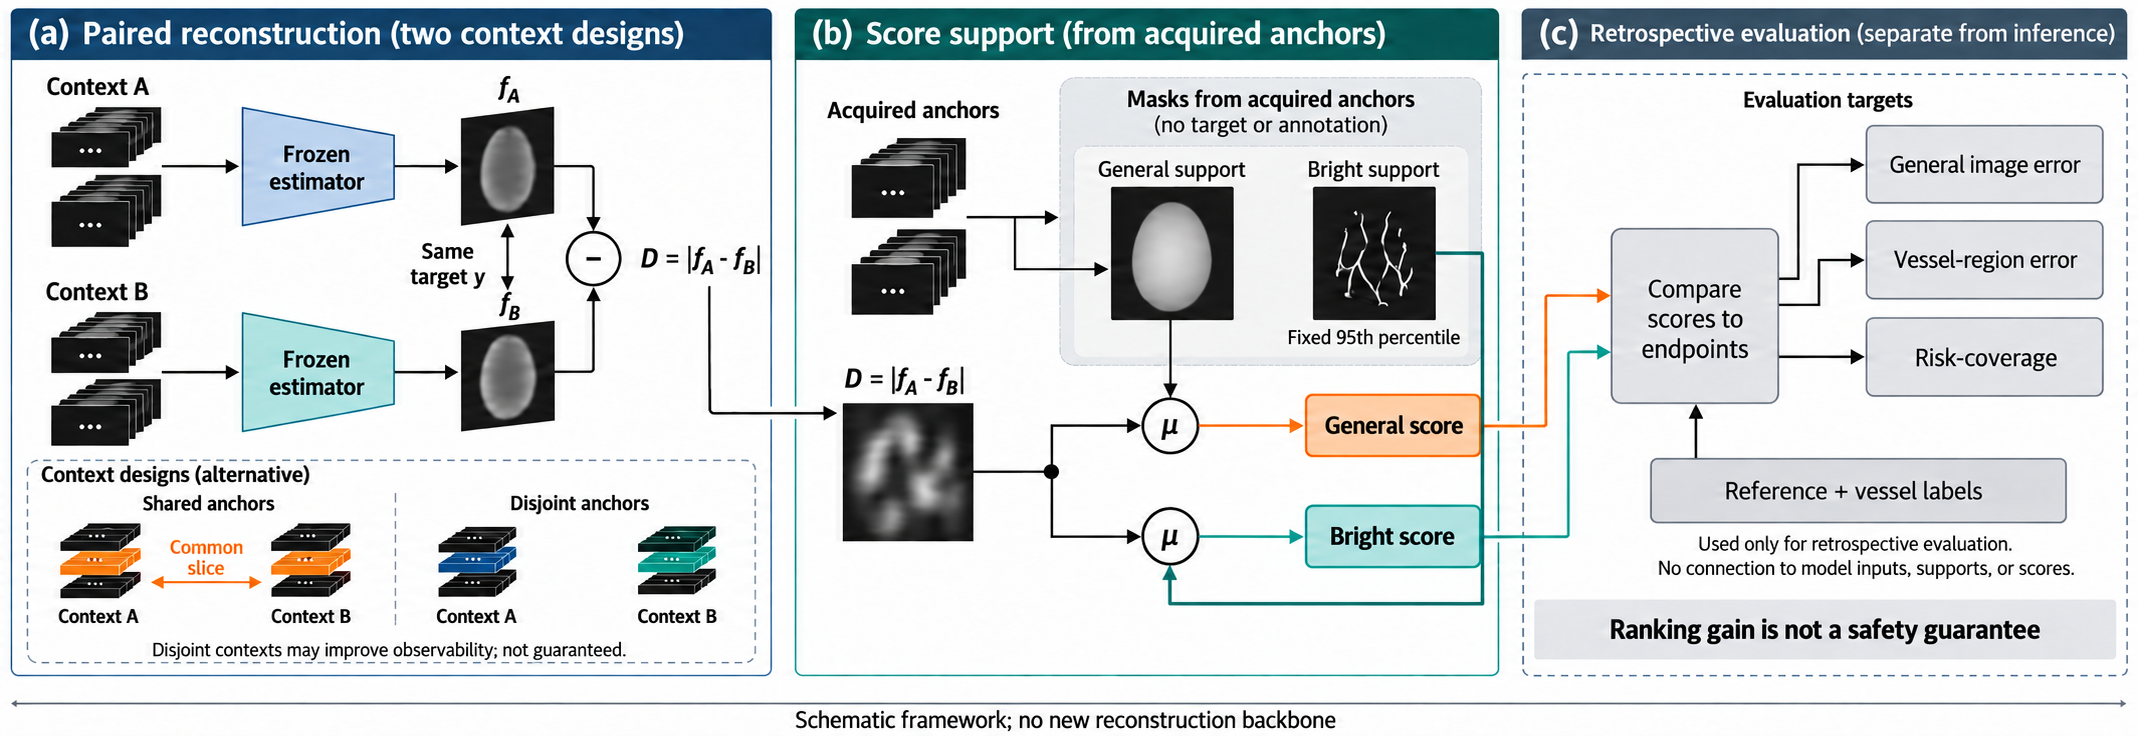
\includegraphics[width=.98\textwidth]{p16_tmi_framework.png}
\caption{Paired-reconstruction framework with acquired-support MRA scoring. General and bright masks independently pool disagreement; references and vessel labels enter retrospective evaluation only. This branch is distinct from historical GT-mask protocols. Images, masks, and model blocks are schematic illustrations, not patient data, measured results, or a new reconstruction backbone.}
\label{fig:concept}
\end{figure*}

\section{Related Work}
Classical splines and learned slice synthesis estimate missing samples from smoothness or anatomical priors \cite{deboor1978splines,peng2020saint,song2024i3net}. Coordinate models such as CycleINR provide a materially different continuous volumetric interpolation paradigm \cite{fang2024cycleinr}. A recent multi-architecture prostate study finds that adjacent-versus-distant input formulation can matter more for reconstruction fidelity than backbone complexity \cite{savant2026formulation}. That study varies the reconstruction problem; we instead hold the target and estimator fixed while intervening on physical measurement identity to study reliability and error cancellation. Leave-one-slice-out evaluation predates this work \cite{horvath2017highorder}; we do not claim the operation as novel. Uncertainty in MRI reconstruction has been studied with variational, Bayesian, posterior-sampling, and ensemble methods \cite{edupuganti2021uncertainty,narnhofer2022bayesian,tanno2021uncertainty,kuestner2024ensembles}. Recent conformal quantile regression estimates pixelwise MRI error intervals \cite{giannakopoulos2026pixelwise}. These methods learn, calibrate, or sample predictive distributions. We instead ask whether deterministic reliability pairs depend on the same physical evidence and explicitly try to falsify the phenomenon across interpolation paradigms.

Ensemble theory distinguishes diversity from accuracy \cite{brown2005diversity,ortega2022diversity}. Our distinction is at the intervention level: target, model, mask, and measurement count remain paired while physical anchor identity changes. This makes dependence observable in a way that arbitrary output transformations do not.

\section{Theory and Hypothesis}
Let the same target $y$ have deterministic predictions $f_a=y+e_a$ and $f_b=y+e_b$. Their squared disagreement is
\begin{equation}
\|f_a-f_b\|^2=\|e_a\|^2+\|e_b\|^2-2\langle e_a,e_b\rangle.\label{eq:cov}
\end{equation}
Positive error alignment suppresses observable disagreement. With $\bar e=(e_a+e_b)/2$ and $\delta=(e_a-e_b)/2$,
\begin{equation}
\tfrac12(\|e_a\|^2+\|e_b\|^2)=\|\bar e\|^2+\|\delta\|^2.\label{eq:decomp}
\end{equation}
We call these shared and observable energy. Shared fraction is $q=\|\bar e\|^2/(\|\bar e\|^2+\|\delta\|^2)$. This is an algebraic retrospective decomposition, not a calibrated uncertainty partition.

No disagreement score alone identifies error. If $e_a=e_b=c\ne0$, disagreement is zero while all error is shared. Conversely, by the triangle inequality, large disagreement implies at least one prediction is inaccurate but does not identify which. Our directional hypothesis is therefore scoped: reducing overlap of error-generating measurements should lower error alignment, increase observable fraction, and improve error ranking, but low disagreement cannot certify correctness.

At factor four, phase-0 anchors are $z=0,4,8,\ldots$ and phase-2 anchors are $z=2,6,10,\ldots$. Targets with $z\bmod4\in\{1,3\}$ are missing from both lattices and the lattices are disjoint (Fig.~\ref{fig:design}). The maximal-shared control reuses phase-0 anchors, reverses their through-plane order, and maps predictions back to physical $z$. It preserves anchor identity but changes order; the design is a paired intervention with a residual order-equivariance confound, not pure identification of an overlap coefficient.

\begin{figure}[t]
\centering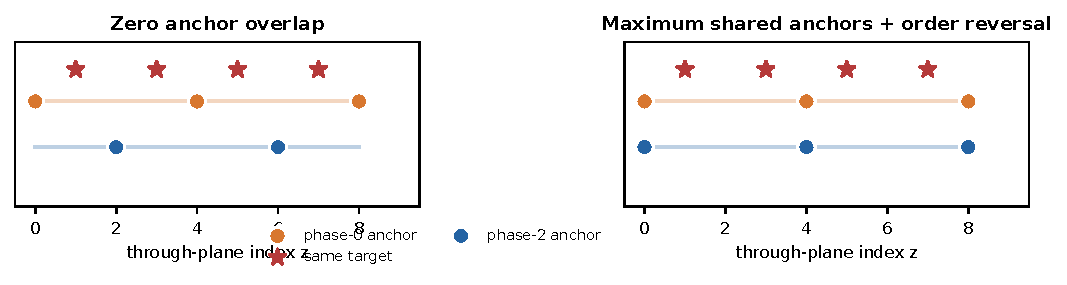
\includegraphics[width=\columnwidth]{fig2_design.pdf}
\caption{Target-preserving $\times4$ design. Stars are evaluated physical planes. Disjoint phase lattices share no anchors; the maximal-shared control reuses the same anchors under reversal.}
\label{fig:design}
\end{figure}

\section{Materials and Methods}
\subsection{Cohorts and Reconstruction}
fastMRI brain T2 used a frozen 112/24/24 split; the 24-case test set enters analysis \cite{zbontar2018fastmri,knoll2020fastmri}. IXI contributed 115 held-out brain T2 examinations \cite{ixi_dataset}. NingXia contributed 22 knee T2 series from eight patients. Its HAT/SwinIR predictions were out of fold under eight patient-group folds, and inference resamples patients rather than series.

Frozen 2.5-D HAT and SwinIR interpolators generated the original three-cohort contexts; that historical analysis uses the through-plane reversal control and retains its stated order-equivariance limitation. No model was refit for reliability. The architecture extension instead uses a clean in-plane horizontal flip mapped back to the target, preserving physical anchor order and geometry. Complete original sources validly evaluate HAT, SwinIR, I3Net, an adapted locally trained SAINT-style conditional CNN, and an internal CycleINR-style coordinate model on all 24 fastMRI and 115 IXI examinations. These labels describe architectural lineage rather than exact official checkpoints. Five residue-balanced missing targets per examination use phase-0 anchors $\{0,4,8,12\}$ and disjoint phase-2 anchors $\{2,6,10,14\}$ where available. Phase-0 reproduction is exact on all 24 fastMRI examinations per model and one frozen IXI examination per model. An independent factor experiment used analytical interpolation in shallow volumes at $\times6$.

\begin{table}[t]
\caption{Cohorts and experimental roles}
\label{tab:data}\centering
\begin{tabular}{lrrp{3.0cm}}
\toprule
Cohort&Cases&Clusters&Role\\
\midrule
fastMRI brain&24&24&Neural overlap, factors, risk\\
IXI brain&115&115&Neural overlap, factors, risk\\
NingXia knee&22&8&OOF overlap, factors, risk\\
\bottomrule
\end{tabular}
\end{table}

\subsection{Physical Matching and Scores}
Generated planes were matched within the recorded grids. A new DICOM audit verifies pixel order and physical positions for all 24 fastMRI test cases; the legacy diagonal affine does not preserve patient orientation. Shapes, orientation codes, affines, plane-normal angles, and distances were audited. Acquired anchors were excluded. For paired predictions $a,b$, the score is mean $|a-b|$ on the declared foreground mask. Plan 9/11 scores use a target-derived 1\% mask. Candidate-bank scores instead use a target-model prediction mask; raw-output recomputation verifies this distinction. The clean legacy flip analysis uses a phase-0 prediction mask. Acquired-anchor scores use only observed slices. These are retrospective evaluations, not uniformly target-free pipelines.

Endpoints were MAE, RMSE, MSE, $1-\mathrm{SSIM}$, gradient MAE, Gaussian low-frequency MAE, and high-frequency residual MAE. The strict stable-wrong definition combined pooled within-dataset/model top-quartile plane MAE and bottom-quartile disagreement. Examination scores were aggregated over matched planes.

For paired errors, total energy was $T=(\|e_a\|^2+\|e_b\|^2)/2$, shared energy $S=\|\bar e\|^2$, and observable energy $O=\|\delta\|^2$. We verified $T=S+O$ before computing fractions. The stored normalized statistic is $D_1=\mathrm{MAE}(a-b)/\sqrt{T}$, not RMSE disagreement. It obeys
\begin{equation}
D_1=2\kappa\sqrt{1-q},\qquad
\kappa=\frac{\mathrm{MAE}(a-b)}{\mathrm{RMSE}(a-b)}\in[0,1].
\label{eq:coupling}
\end{equation}
For nonzero disagreement, $\kappa$ describes residual shape. Thus the normalized-disagreement/shared-fraction association is structurally coupled and cannot independently validate the mechanism.

Three intensity strategies were prespecified. Raw scale preserves the stored computation. Pooled-common normalization applies one robust affine transform to both predictions and target within a case. Independent-output normalization transforms each prediction separately and is a negative control: it can remove amplitude failures differently and therefore does not preserve an absolute paired residual.

The IXI identity-swap control matches the nearest-anchor distance multiset $\{1,3\}$ up to left--right reflection. Residues $z\bmod4=1$ and 3 are summarized separately and then weighted equally. A bootstrap interval for their difference that excludes zero is defined as an orientation warning. This removes residue imbalance but establishes reflection-equivalent, not identical signed, target geometry.

The selective-risk endpoint was independently stored mean HAT/SwinIR $\times4$ examination MAE. Comparators were measurement-disjoint disagreement, maximal-shared disagreement, HAT--SwinIR committee disagreement, and adjacent-anchor MAE. After sorting from low to high score, risk $R(c)$ is retained mean endpoint error at coverage $c$. Normalized AURC subtracts oracle AURC and divides by reverse-oracle minus oracle AURC; lower is better \cite{ding2020selective}.

\subsection{Statistical Analysis}
Spearman correlation measures ordering, not calibration. Primary intervals used 5,000 cluster bootstrap replicates, resampling 24 fastMRI examinations, 115 IXI examinations, or eight NingXia patients with subordinate planes/models retained. Partial rank analyses residualized shared fraction and disagreement against total error and examination indicators. Multi-endpoint confirmation required a positive disjoint-minus-shared direction for a majority of justified endpoints in every eligible cohort; all endpoints are reported. No universal superiority or clinical-safety test is performed.

The endpoint and score are paired by dataset, case, model, and physical plane. Bootstrap samples carry both contexts together, so their difference is recomputed rather than treating correlations as independent. We report point-estimate unanimity but do not count 42 correlated rows as independent discoveries. Complete risk curves complement correlation because the high-risk tail can differ even when overall ranks are similar.

The exploratory sensitivity analysis uses 10,000 paired cluster bootstrap replicates and five-model simultaneous intervals from the bootstrap maximum absolute standardized deviation. A same-label densification comparison can use different factor-specific checkpoints. Benefit is common-support $\mathrm{MAE}_{\times4}-\mathrm{MAE}_{\times2}$ for the same dataset, case, fold, model, and support. Every model with finite paired errors is eligible. Frozen scores are Anchor-CV, adjacent-anchor MAE, and median $\times4$ target-model disagreement against registry-declared candidate-bank members. Inference is reported separately by dataset and model with examination/patient-cluster bootstrap; the analysis is exploratory because the underlying reconstruction outputs already existed.

\section{Results}
\subsection{Original All-Plane Paired Intervention}
Before the common three-plane Plan6 analysis, the frozen all-eligible-plane experiment established the target-preserving contrast on fastMRI and NingXia (Fig.~\ref{fig:original}). On fastMRI, zero-overlap disagreement correlated with phase-0 MAE at $\rho=0.960$, versus 0.605 for the maximal-shared control, a paired difference of 0.355 (case-clustered 95\% CI 0.225--0.557). On NingXia, correlations were 0.891 and 0.699, a difference of 0.193. Correct resampling of eight patient groups gave CI 0.113--0.336.

The effect was positive for each architecture: fastMRI HAT/SwinIR differences were 0.340/0.375 and NingXia differences 0.128/0.258. The endpoint, mask, model, target plane, and number of anchors were paired. Raw disagreement magnitude did not explain the result: on fastMRI, disjoint raw disagreement was only 59.1\%/77.2\% of maximal-shared disagreement for HAT/SwinIR despite much better error ranking. NingXia had the opposite magnitude ordering. Output diversity magnitude is therefore neither necessary nor sufficient for error observability.

The later three-plane computation uses equal examination coverage and adds IXI plus six endpoints. Its smaller pooled MAE advantages (0.117/0.086/0.185) are not a failed replication of the historical statistic; they reflect a different, prespecified balanced sampling estimand. Both analyses retain the same direction.

\begin{figure}[t]
\centering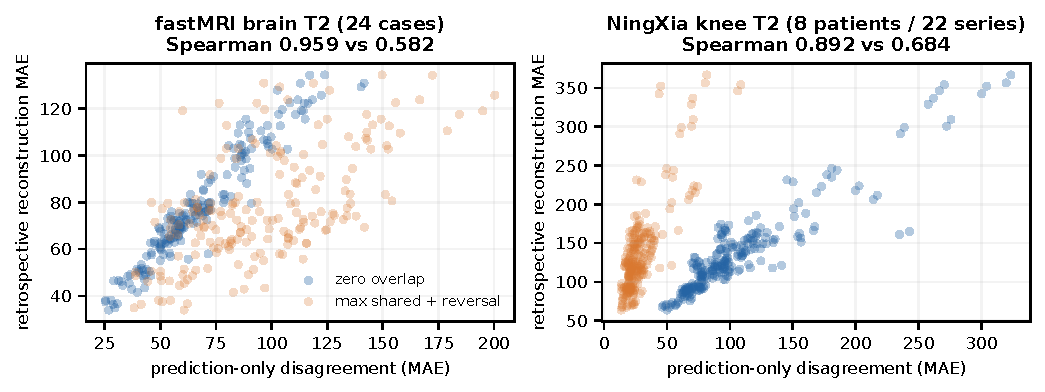
\includegraphics[width=\columnwidth]{fig3_main_overlap.pdf}
\caption{Frozen all-plane paired intervention. Measurement-disjoint scores rank the same stored target error more strongly than the maximal-shared reversal control. Inference clusters examinations/patients.}
\label{fig:original}
\end{figure}

\subsection{Shared Error Suppresses Observability}
Across every cohort, architecture, and context, shared fraction had a strong negative partial association with MAE disagreement normalized by paired-error RMS after controlling total error and examination: $-0.746$ to $-0.923$ on fastMRI, $-0.806$ to $-0.975$ on IXI, and $-0.894$ to $-0.959$ on NingXia (Fig.~\ref{fig:consensus}). These are descriptive associations constrained by Eq.~\ref{eq:coupling}, not independent tests of error cancellation. The stored MAE normalization factorizes to numerical precision after retaining the residual-shape term.

Strict stable-wrong prevalence was zero for disjoint contexts. Under maximal sharing it was zero on fastMRI, 0.28--0.32\% on IXI, and 2.42--3.23\% on NingXia. Patient-clustered NingXia intervals were wide. The failure is coherent but rare under this definition.

The prevalence calculation uses one pooled threshold per dataset/model across both contexts, preventing each condition from defining its own easy quartile. IXI HAT increased by 0.324 percentage points (clustered CI 0.014--0.865); other intervals included zero. NingXia upper limits reached 6.6--8.8\%. These estimates reject both extreme interpretations: shared contexts do permit high-error/low-disagreement planes, but the current strict phenotype is not common enough to estimate a clinical incidence.

\begin{figure}[t]
\centering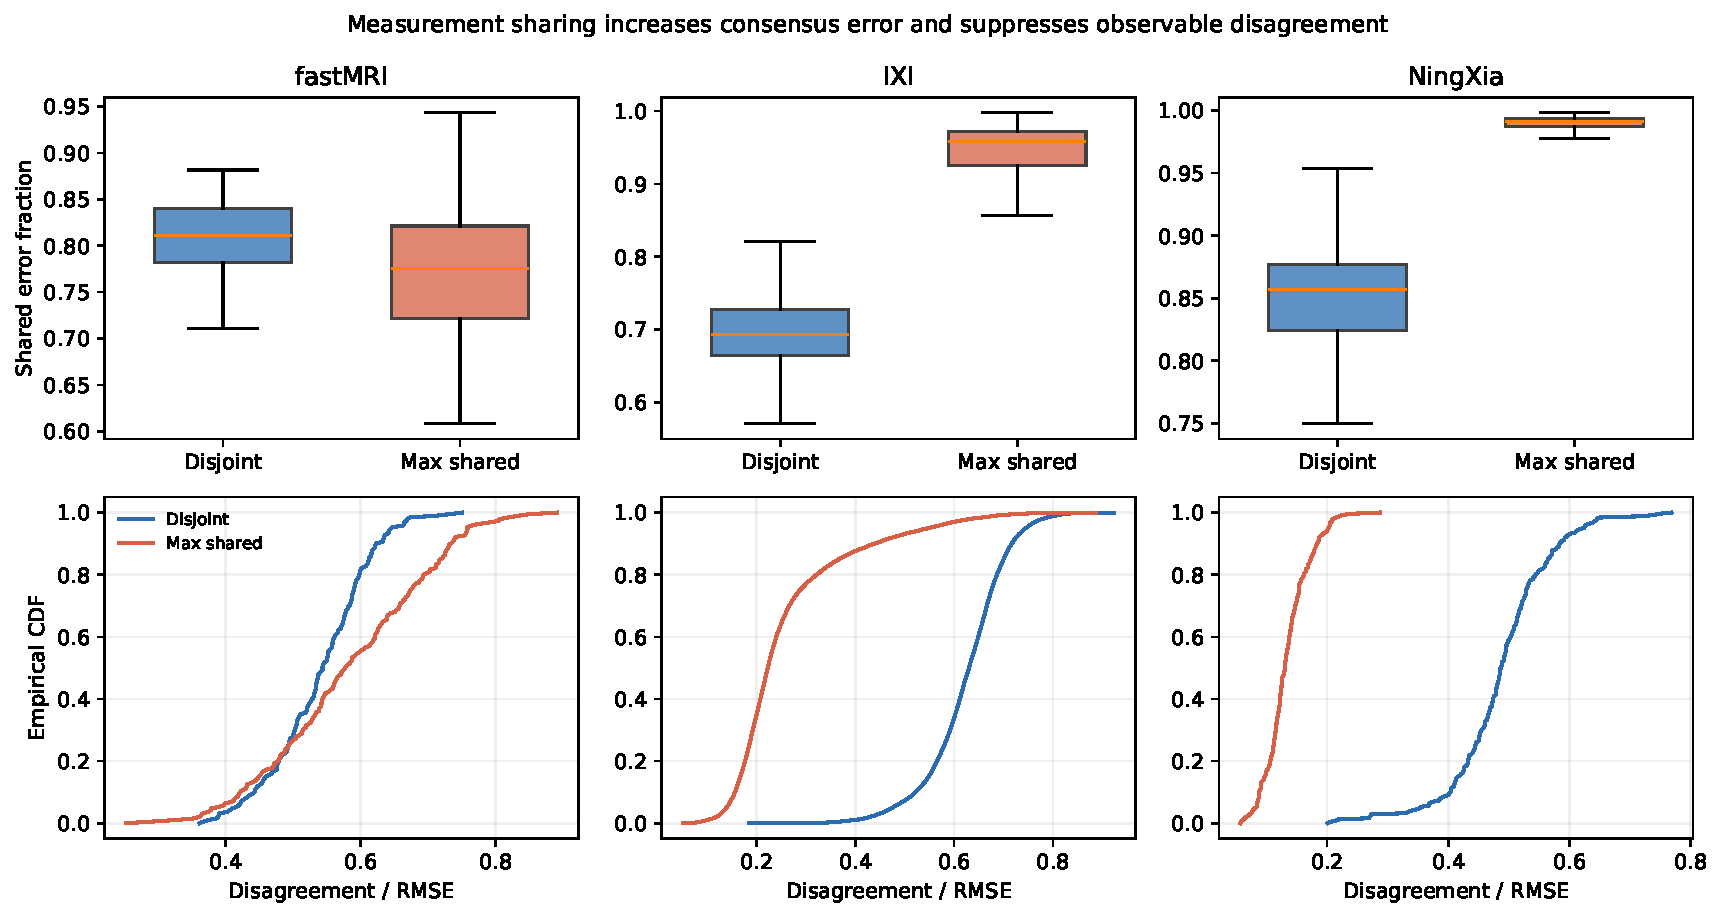
\includegraphics[width=\columnwidth]{p6_e02_consensus_distributions.pdf}
\caption{Consensus distributions and normalized disagreement across contexts. The distributions describe error allocation; normalized disagreement and shared fraction are structurally coupled by Eq.~\ref{eq:coupling}.}
\label{fig:consensus}
\end{figure}

\subsection{Seven Endpoints and Two Architectures}
All 42 dataset--architecture--endpoint point differences favored disjoint contexts (Fig.~\ref{fig:metrics}). Architecture-pooled disjoint/shared correlations for MAE were 0.957/0.840 (fastMRI), 0.977/0.891 (IXI), and 0.862/0.676 (NingXia). RMSE differences were 0.193/0.083/0.210; low-frequency differences were 0.123/0.103/0.198. The direction persisted separately for HAT and SwinIR.

Structural error is the main boundary. SSIM-error correlations were near zero on fastMRI and negative on NingXia for both contexts, although their disjoint-minus-shared differences remained positive. Only IXI had consistently positive SSIM ranking and intervals excluding zero. Some gradient/high-frequency intervals also crossed zero in smaller strata. Pixelwise disagreement therefore ranks broad intensity error but is not a universal structural-error surrogate.

Table~\ref{tab:endpoints} reports architecture-pooled estimates without endpoint selection. Low-frequency error closely follows MAE, indicating that the result is not driven only by edge noise. The SSIM rows show why direction and absolute utility must be separated: a positive difference can mean ``less poor'' rather than useful structural-error ranking.

A prespecified Plan7 contrast tested whether blindness was systematically stronger for intensity/low-frequency endpoints than for structural/high-frequency endpoints. It was not: the family contrast was negative for IXI HAT/SwinIR ($-0.068/-0.074$, clustered intervals below zero), positive for NingXia ($0.064/0.063$, one interval crossing zero), and uncertain on fastMRI. Endpoint heterogeneity is therefore cohort dependent; the data support neither metric independence nor a universal frequency-family mechanism.

\begin{table*}[t]
\caption{Architecture-pooled Spearman correlations for every Plan6 endpoint}
\label{tab:endpoints}\centering
\begin{tabular}{llrrr@{\quad}llrrr}
\toprule
Cohort&Endpoint&Disjoint&Shared&$\Delta$&Cohort&Endpoint&Disjoint&Shared&$\Delta$\\
\midrule
fastMRI&MAE&.957&.840&.117&IXI&MAE&.977&.891&.086\\
&RMSE&.936&.743&.193&&RMSE&.972&.888&.083\\
&MSE&.936&.785&.151&&MSE&.971&.889&.082\\
&SSIM error&.006&$-.070$&.076&&SSIM error&.417&.081&.336\\
&Gradient&.640&.423&.217&&Gradient&.973&.908&.065\\
&Low frequency&.960&.836&.123&&Low frequency&.975&.872&.103\\
&High frequency&.562&.372&.189&&High frequency&.969&.891&.079\\
\midrule
NingXia&MAE&.862&.676&.185&&&&&\\
&RMSE&.807&.597&.210&&&&&\\
&MSE&.807&.597&.210&&&&&\\
&SSIM error&$-.240$&$-.326$&.086&&&&&\\
&Gradient&.629&.468&.161&&&&&\\
&Low frequency&.864&.666&.198&&&&&\\
&High frequency&.642&.479&.164&&&&&\\
\bottomrule
\end{tabular}
\end{table*}

\begin{figure}[t]
\centering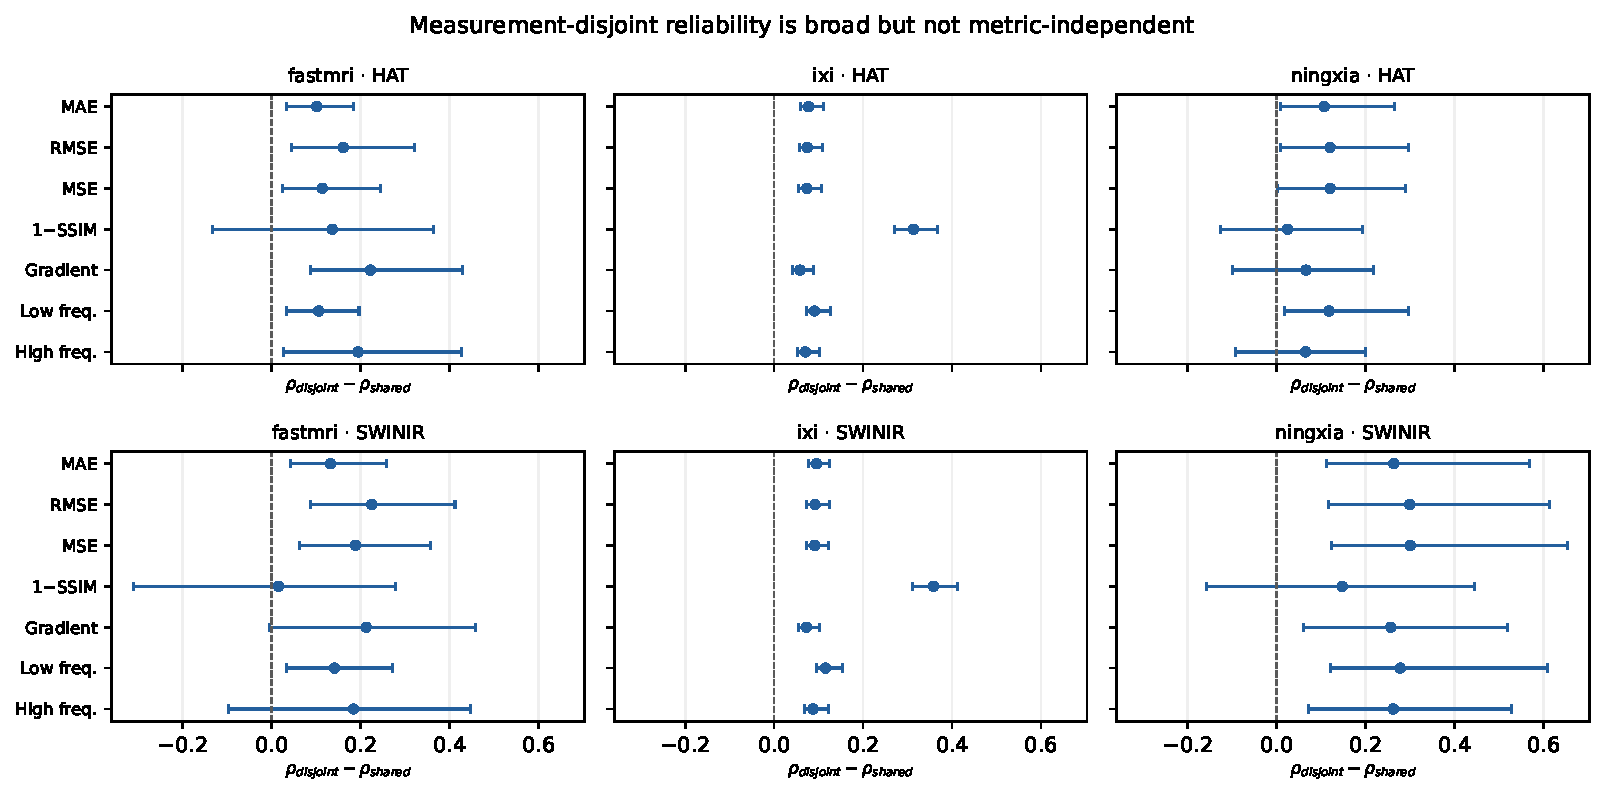
\includegraphics[width=\columnwidth]{p6_e01_metric_robustness.pdf}
\caption{Seven-endpoint disjoint-minus-shared Spearman differences with examination/patient-clustered intervals. All point estimates are positive; structural/frequency uncertainty is retained.}
\label{fig:metrics}
\end{figure}

\subsection{Factor, Geometry, and Intensity Robustness}
From $\times2$ to $\times6$, mean shared fraction increased $0.843\rightarrow0.953$ on fastMRI, $0.750\rightarrow0.923$ on IXI, and $0.860\rightarrow0.953$ on NingXia (Fig.~\ref{fig:factors}). Reliability decreased $0.955\rightarrow0.798$, $0.961\rightarrow0.947$, and $0.937\rightarrow0.818$, respectively. Paired MAE increased in all cohorts while absolute disagreement generally decreased; IXI had a small $\times6$ rebound without reliability recovery. The factor phenomenon therefore occurs in transparent analytical estimators and is not exclusively neural.

Across 322 $\times4$ HAT/SwinIR output volumes, shapes, orientations, and affines were identical. All physical planes matched at every tolerance from $10^{-6}$ to $10^{-1}$ mm; maximum affine and plane-distance differences were zero. Applying one shared per-case robust transform to predictions and target preserved a positive disjoint-minus-shared contrast in all six architecture--cohort strata (0.121--0.700). It did not preserve cross-examination ranks, especially on IXI. Independent output normalization changed ranks further and is invalid for absolute discrepancy.

\begin{figure}[t]
\centering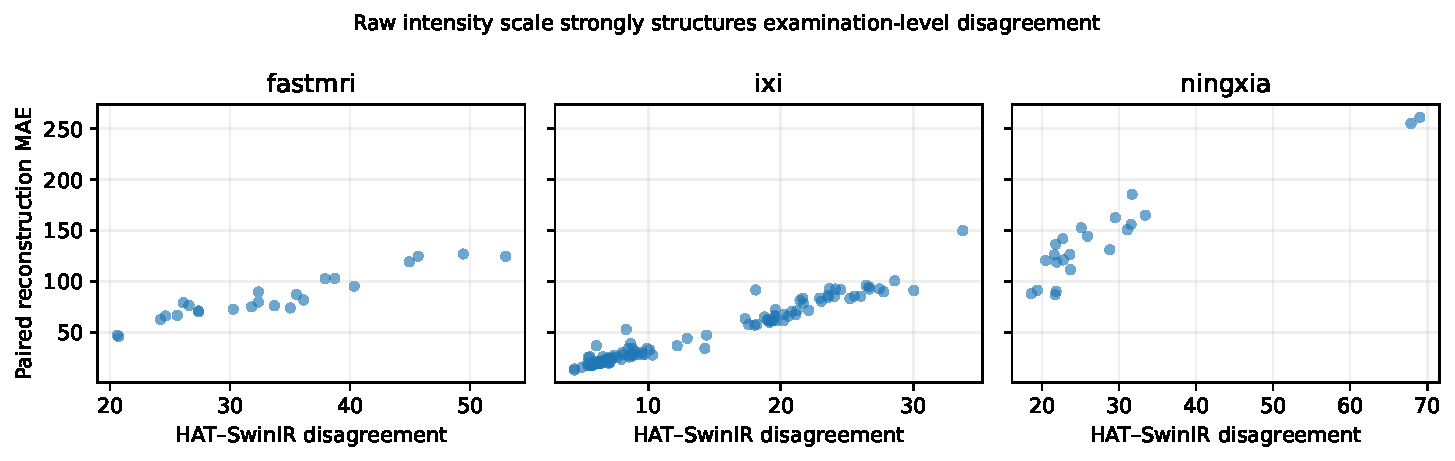
\includegraphics[width=\columnwidth]{p6_e03_intensity_audit.pdf}
\caption{Intensity operating range. A shared case transform preserves the paired overlap direction but can change cross-examination ranks; independent output transforms are not a valid absolute-discrepancy control.}
\label{fig:intensity}
\end{figure}

\begin{table}[t]
\caption{Analytical factor response}
\label{tab:factors}\centering
\begin{tabular}{llrrr}
\toprule
Cohort&Metric&$\times2$&$\times4$&$\times6$\\
\midrule
fastMRI&Pair MAE&112.1&137.6&151.8\\
&Shared fraction&.843&.940&.953\\
&Reliability $\rho$&.955&.833&.798\\
IXI&Pair MAE&49.8&67.4&82.8\\
&Shared fraction&.750&.886&.923\\
&Reliability $\rho$&.961&.947&.947\\
NingXia&Pair MAE&157.1&186.2&214.6\\
&Shared fraction&.860&.933&.953\\
&Reliability $\rho$&.937&.830&.818\\
\bottomrule
\end{tabular}
\end{table}

The geometry audit rules out tolerance-induced membership changes: normal-angle differences were at most $1.48\times10^{-6}$ degrees and physical distance was zero. The intensity audit instead establishes an operating boundary. Raw committee disagreement correlated with examination error by 0.923/0.957/0.874 across the cohorts. A per-case common transform reduced these to 0.784/0.256/0.239. The within-case overlap direction is robust, but between-case triage requires a declared common scale.

\begin{figure}[t]
\centering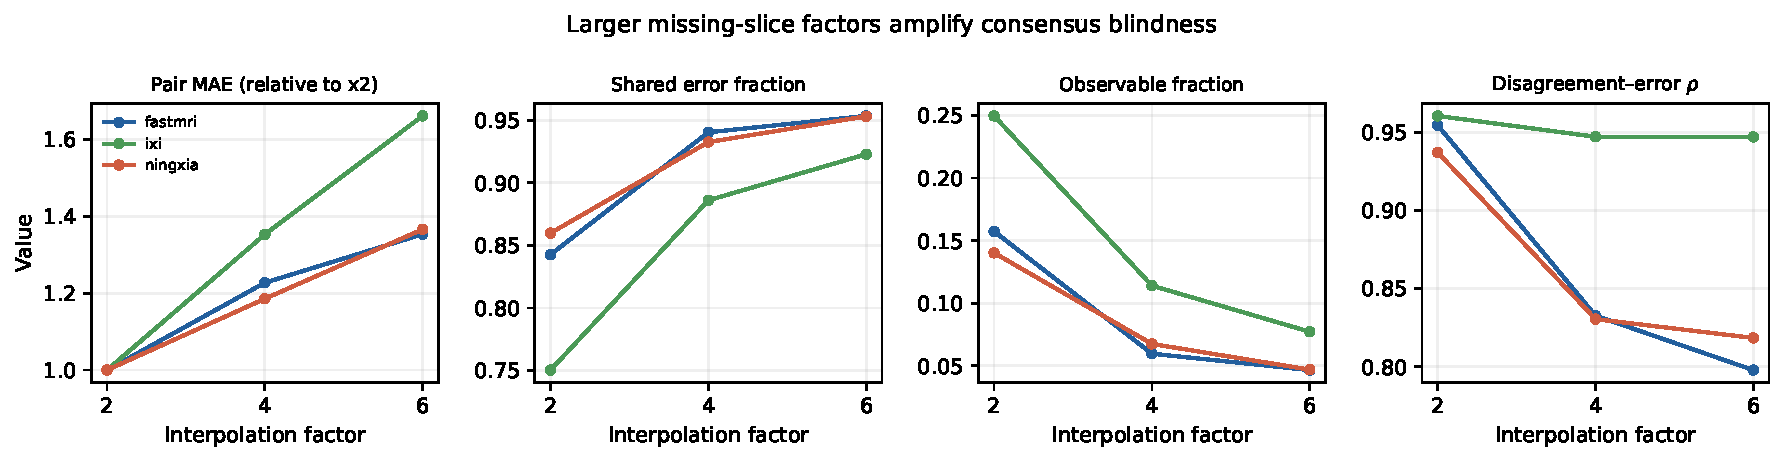
\includegraphics[width=\columnwidth]{p6_e11_factor_robustness.pdf}
\caption{Analytical factor response. As missing-slice factor increases, error and shared fraction rise while observable fraction and disagreement reliability fall in every cohort.}
\label{fig:factors}
\end{figure}

\subsection{Selective Risk}
Table~\ref{tab:risk} and Fig.~\ref{fig:risk} report complete examination-level curves. Measurement-disjoint nAURC was 0.0119/0.0013/0.0107 on fastMRI/IXI/NingXia, substantially lower than maximal-shared and committee disagreement in every cohort. It was not universally best: adjacent-anchor MAE achieved 0.0070 on NingXia. Disjoint scoring is the most reliable tested output-based construction, whereas a cheaper input statistic can win in an external cohort.

At fixed coverage, disjoint IXI risk was 16.58 at 10\% versus oracle 16.55 and was exactly oracle (21.70) at 50\%. On fastMRI, several methods selected the same easiest small subset but diverged at intermediate coverage: disjoint 50\% risk was 63.65, compared with 65.36 maximal-shared and 65.97 adjacent-anchor. On NingXia, adjacent MAE improved 50\% risk from 111.24 to 109.30. No threshold is chosen because clinical capacity and error costs were not specified.

Architecture disagreement is not independent of case difficulty. HAT--SwinIR case-error rank correlations were 0.989/1.000/0.997, and examination identity accounted for 99.1\%/99.99\%/99.78\% of two-architecture squared-error variation. Two architectures can therefore agree about which cases are hard while sharing the dominant error. This explains why committee disagreement is a strong baseline yet remains dependence preserving.

We also counted operational false retention using a threshold frozen as the top quartile of the common examination error and fixed 30/50/70/90\% coverages. At 70\% coverage, measurement-disjoint scoring retained 0 of 6 high-error fastMRI examinations, compared with 1/0/1 under maximal-shared, committee, and adjacent-anchor scores. On IXI it retained 0 of 29, compared with 2/1/3; the disjoint advantage over maximal-shared and adjacent scores was 0.069 (95\% clustered CI 0--0.167) and 0.103 (0--0.188). All NingXia methods retained 1 of 6 at this coverage, with wide patient-clustered intervals. At 90\% coverage scores converged because capacity forced most examinations to remain. Thus the operational benefit is concentrated at intermediate coverage and is strongest in IXI; it is not a universal threshold or clinical miss rate.

\begin{table}[t]
\caption{High-error examinations retained at 70\% coverage}
\label{tab:false-retention}\centering
\begin{tabular}{lrrr}
\toprule
Score&fastMRI&IXI&NingXia\\
\midrule
Measurement-disjoint&0&0&1\\
Maximal-shared&1&2&1\\
Architecture committee&0&1&1\\
Adjacent-anchor MAE&1&3&1\\
\bottomrule
\end{tabular}
\end{table}

\begin{table}[t]
\caption{Examination-level reliability (lower nAURC is better)}
\label{tab:risk}\centering
\begin{tabular}{lrrr}
\toprule
Score&fastMRI&IXI&NingXia\\
\midrule
Measurement-disjoint&.0119&.0013&.0107\\
Maximal-shared&.0684&.0139&.0306\\
Architecture committee&.0193&.0140&.0504\\
Adjacent-anchor MAE&.0212&.0143&\textbf{.0070}\\
\bottomrule
\end{tabular}
\end{table}

\begin{figure}[t]
\centering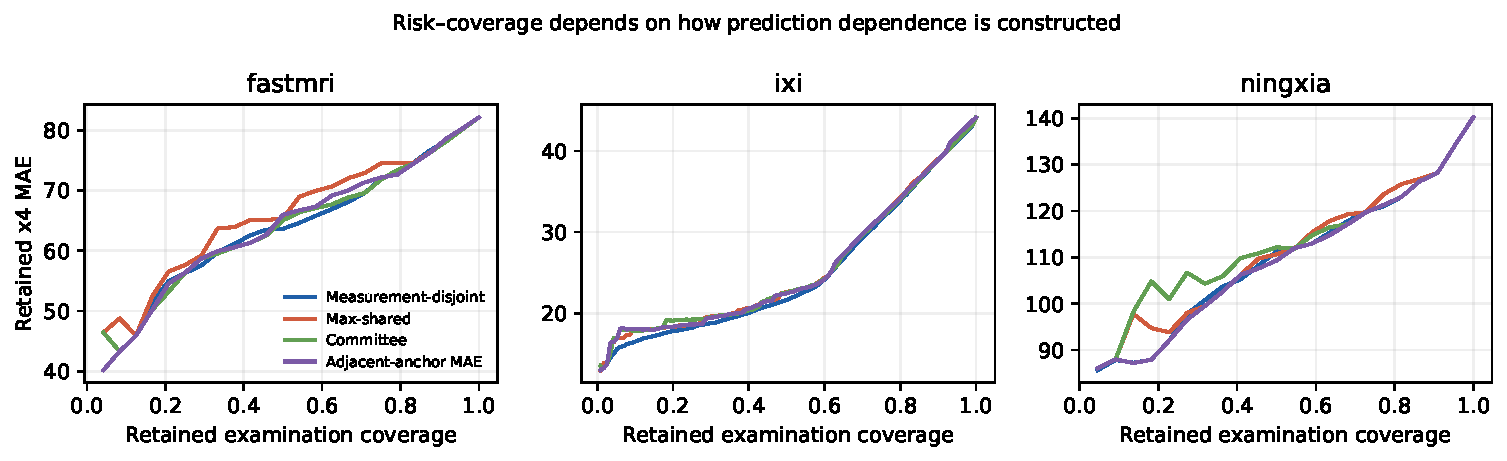
\includegraphics[width=\columnwidth]{p6_e12_risk_coverage.pdf}
\caption{Risk--coverage against one stored mean HAT/SwinIR MAE endpoint. Disjoint disagreement beats dependence-preserving output scores in all cohorts; adjacent-anchor MAE wins on NingXia.}
\label{fig:risk}
\end{figure}

\subsection{Retrospective Densification Consequence}
A score can rank current error without identifying incremental benefit. We evaluate stored $\times4\rightarrow\times2$ improvement with matched model labels and common target support; this does not fix factor-specific learned weights. The common-support audit includes all 13 eligible models on fastMRI and NingXia rather than selecting a favorable architecture.

Anchor-CV has positive within-model association with benefit for 13/13 fastMRI models and 12/13 NingXia models, with median $\rho=.851/.727$. Adjacent-anchor MAE gives 13/13 and 12/13 (median .802/.748), while candidate-bank disagreement gives 11/11 and 10/11 (.835/.710); its denominator reflects neural-only target precomputation, although Linear/Cubic are bank members. The only non-positive model is the severely degraded NingXia Res-SRDiff run, whose three intervals all cross zero. At 10/20/30/50\% budgets, the across-model median oracle-normalized gain is positive for every score and cohort, although individual Res-SRDiff policies can fall below random.

Since benefit contains current $\times4$ error, we also condition on its rank. Anchor-CV median partial correlation falls from .851/.727 to .203/.291 on fastMRI/NingXia; all 26 model--cohort intervals cross zero. This weakens a claim of incremental benefit information beyond current difficulty.

We additionally recover a same-architecture I3Net pair on all 115 IXI examinations. Different $\times2/\times4$ checkpoint hashes are recorded. Re-evaluation uses 7,334 common odd planes, identical target-derived masks and physical affines; case means are computed before examination bootstrap. Mean MAE falls from 33.65 to 25.62, with positive benefit in 115/115 cases. Linear interpolation on the same support gives 57.36 and 39.21. Raw Anchor-CV and adjacent MAE correlate with benefit at .843 [.768,.894] and .845 [.771,.896]; conditional correlations are .216 [.007,.430] and .227 [.020,.437]. These are pointwise exploratory intervals.

Normalization by the acquired-anchor robust range reverses the raw-benefit correlations to $-.238$ [$-.404,-.058$] and $-.236$ [$-.397,-.060$]. At 50\% selection, normalized Anchor-CV is below random by .920 MAE units (95\% CI $[-1.635,-.149]$). This is a scale-sensitive ranking failure against a raw-scale endpoint, not a claim that normalization is always harmful. Normalizing both score and benefit by the same acquired range gives correlations .539 [.356,.698] and .551 [.372,.704]; raw scores against normalized benefit instead give $-.375/-.373$. The four contracts preserve both positive and negative results: a shared denominator can itself induce association, so this is a unit-sensitivity diagnostic, not a new calibrated score.

Independent source reconstruction also distinguishes prediction-only bank support from GT support. Across all 11 neural targets, acquired-input masks yield median raw benefit correlations .863/.723 on fastMRI/NingXia, compared with .835/.710 for prediction masks and .805/.519 for bank unions. Current-error-adjusted medians remain $-.058/.425$ for acquired masks. Changing support does not remove the current-difficulty limitation.



\subsection{Complete Baseline Comparison and Budget Sensitivity}
Table~\ref{tab:p15-master} restores all 13 methods on all three $\times4$ cohorts: classical, CNN, GAN, Transformer, INR, Mamba, ACVTT, and diffusion-refinement baselines. We independently reproduce every original PSNR/SSIM/MAE/MSE/NCC entry. I3Net leads all five metrics on IXI/fastMRI, whereas SwinIR leads four on NingXia and HAT leads NCC. The complete supplement retains 111 configurations: 39 at $\times4$, 52 at $\times2/\times6$, and 20 longer-budget results. Native full-plane metrics and eight-fold NingXia averaging differ from the masked common-support QA contract and are never interchanged.

\begin{table*}[t]
\caption{All 13 master-table baselines at $\times4$, independently recovered from original metrics. PSNR/SSIM are higher-is-better; MAE is lower-is-better. Full-plane evaluation excludes acquired planes. IXI/fastMRI average examinations; NingXia averages eight patient folds. These values do not replace the masked common-support reliability endpoints.}
\label{tab:p15-master}\centering\small\setlength{\tabcolsep}{3.7pt}
\begin{tabular}{lrrrrrrrrr}\toprule
&\multicolumn{3}{c}{IXI (115)}&\multicolumn{3}{c}{fastMRI (24)}&\multicolumn{3}{c}{NingXia (8 folds)}\\
Method&PSNR&SSIM&MAE&PSNR&SSIM&MAE&PSNR&SSIM&MAE\\\midrule
Linear & 26.17 & 0.853 & 29.28 & 19.11 & 0.597 & 78.81 & 22.73 & 0.675 & 103.21\\
Cubic & 25.71 & 0.842 & 31.13 & 17.97 & 0.533 & 91.93 & 21.65 & 0.618 & 119.41\\
ACVTT & 27.34 & 0.882 & 25.52 & 20.19 & 0.662 & 71.55 & 23.47 & 0.728 & 95.44\\
Res-SRDiff & 28.04 & 0.882 & 24.19 & 21.67 & 0.691 & 56.34 & 21.15 & 0.554 & 153.02\\
ArSSR & 27.25 & 0.877 & 25.55 & 20.31 & 0.657 & 65.99 & 23.16 & 0.709 & 96.49\\
CycleINR-style & 26.17 & 0.853 & 29.28 & 20.32 & 0.658 & 66.10 & 22.90 & 0.693 & 101.10\\
ResUNet & 27.46 & 0.881 & 25.24 & 22.25 & 0.737 & 53.57 & 23.38 & 0.721 & 97.04\\
Pix2Pix-GAN & 27.11 & 0.851 & 27.02 & 21.91 & 0.729 & 53.26 & 22.45 & 0.711 & 105.81\\
SwinIR & 28.65 & 0.900 & 22.46 & 22.36 & 0.749 & 50.87 & 23.95 & 0.752 & 85.97\\
SAINT-style & 28.67 & 0.897 & 22.84 & 23.26 & 0.770 & 46.44 & 23.84 & 0.742 & 89.41\\
I3Net & 31.31 & 0.928 & 17.53 & 24.01 & 0.792 & 41.01 & 23.49 & 0.721 & 93.57\\
HAT & 28.72 & 0.902 & 22.25 & 23.09 & 0.769 & 47.25 & 23.95 & 0.752 & 86.14\\
SMamba-UNet & 29.35 & 0.908 & 21.14 & 22.73 & 0.762 & 49.45 & 23.91 & 0.750 & 86.82\\
\bottomrule\end{tabular}
\par\smallskip\parbox{.98\textwidth}{\footnotesize Locally adapted implementations retain their recorded training budgets; the master uses extended HAT training on fastMRI. This is not an equal-compute leaderboard. Standard and longer-budget results are reported separately.}
\end{table*}


All 13 models give median case-error rank correlations .997/.899/1.000 on IXI/fastMRI/NingXia (78 pairs each; descriptive). The historical masked seven-stratum audit remains separate: median correlations .938--.991, including a low NingXia diffusion tail. Full-bank evidence therefore supports shared difficulty but not uniformly independent errors.

Crucially, training budget changes the failure interpretation. Across all 20 recorded extensions, 15 paired MAE intervals favor longer training under simultaneous inference; five cross zero. NingXia Res-SRDiff $\times2$ MAE improves 440.61$\rightarrow$140.45$\rightarrow$118.25 at 30/60/90 epochs, still worse than Linear (78.53). The corresponding 60/90-epoch reductions are 300.16 [153.17,447.14] and 322.36 [166.01,478.71]. These separate runs diagnose convergence sensitivity; they do not replace the standard-budget failure or establish an intrinsic diffusion limitation. Profiles retain unequal recorded budgets, including extended fastMRI HAT training. Complete five-metric, multi-scale, and budget tables accompany the baseline supplement.

\subsection{Generalization Across Interpolation Paradigms}
Figure~\ref{fig:arch-generalization} reports the frozen physical-dependence intervention on two independent brain cohorts. On fastMRI, disjoint-minus-shared observable-error gain is 17.8/17.6/8.0/13.7/22.6 points for HAT/SwinIR/I3Net/SAINT/CycleINR; all clustered intervals exclude zero. The IXI replication gives 29.0/30.2/25.2/29.8/29.6 points, with all five intervals above zero and all 115 case effects positive for every model. Its equal-weight four-family estimate is 28.6 points, and leave-one-family-out estimates remain 28.1--29.7 points. Reflection-balanced identity-swap estimates are 29.2/30.0/25.1/29.7/29.5 points; all five mirror-difference intervals include zero. Phase-0 wrapper maximum error is zero for all ten cohort--model runs. Thus local error geometry, rather than examination ranking, is the more reproducible cross-paradigm endpoint.

\begin{figure*}[t]
\centering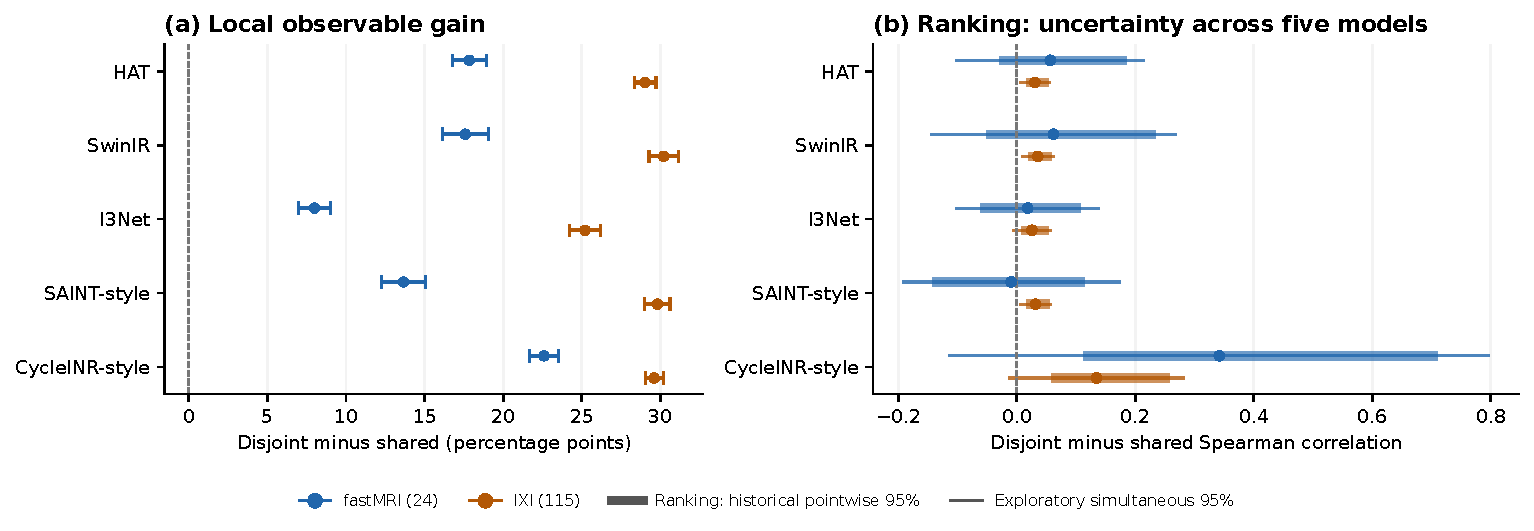
\includegraphics[width=.96\textwidth]{p13_architecture_robustness.pdf}
\caption{Architecture replication and multiplicity sensitivity. (a) Local gains retain positive five-model simultaneous 95\% intervals (10,000 examination bootstraps); fastMRI uses means and IXI medians. (b) Thick bars are historical pointwise intervals; thin bars are simultaneous intervals with within-case median ranking. Simultaneous ranking intervals exclude zero for three IXI models and none on fastMRI. Cohorts are not pooled.}
\label{fig:arch-generalization}
\end{figure*}

The ranking arrow does not generalize uniformly across cohorts. On IXI, $\Delta\rho$ is .031/.035/.025/.032/.134 for HAT/SwinIR/I3Net/SAINT/CycleINR and every interval is positive. On fastMRI, only CycleINR is clearly positive (.342 [.113,.711]); the other four intervals cross zero. The frozen stable-wrong rule yields four of 120 shared fastMRI CycleINR planes and zero for the other models, with zero disjoint CycleINR events. This remains rare. Exploratory five-model simultaneous ranking intervals exclude zero for IXI HAT/SwinIR/SAINT only, and for no fastMRI model. In contrast, all local-gain simultaneous intervals remain positive under four mean/median aggregation choices.

Architectural distance also fails to guarantee examination-level independence. In the prospectively frozen five-model subset, median pairwise case-error rank is .945, .981, and .981 at $\times2/\times4/\times6$; six of 24 cases fall in the top error quartile for all five models at $\times4$ and $\times6$. The exploratory full-bank audit above generalizes the shared-difficulty observation without promoting a new primary endpoint. Pixel geometry is more diverse: median HAT--SwinIR error cosine is .918, versus .564 for CycleINR--I3Net, with corresponding observable fractions .041 and .245. The data therefore distinguish useful local error diversity from the persistent intrinsic difficulty of entire examinations.

\subsection{External MRA and Anatomical Error}
All 125 locally available TopCoW MRA cases have paired vascular annotations~\cite{yang2026topcow}. We use the public challenge training images as a new external evaluation cohort, with no estimator fitting. Fixed linear (L) and four-point Lagrange cubic (C) interpolation use complete native-resolution contexts on phase-0/phase-2 $\times4$ grids. All 10779 eligible odd planes enter; residues 1 and 3 receive equal case weight. The score mask is the union of the two nearest phase-0 acquired-anchor masks. Vessel labels are used only to evaluate error, never to select inputs or target planes.

\begin{figure*}[t]
\centering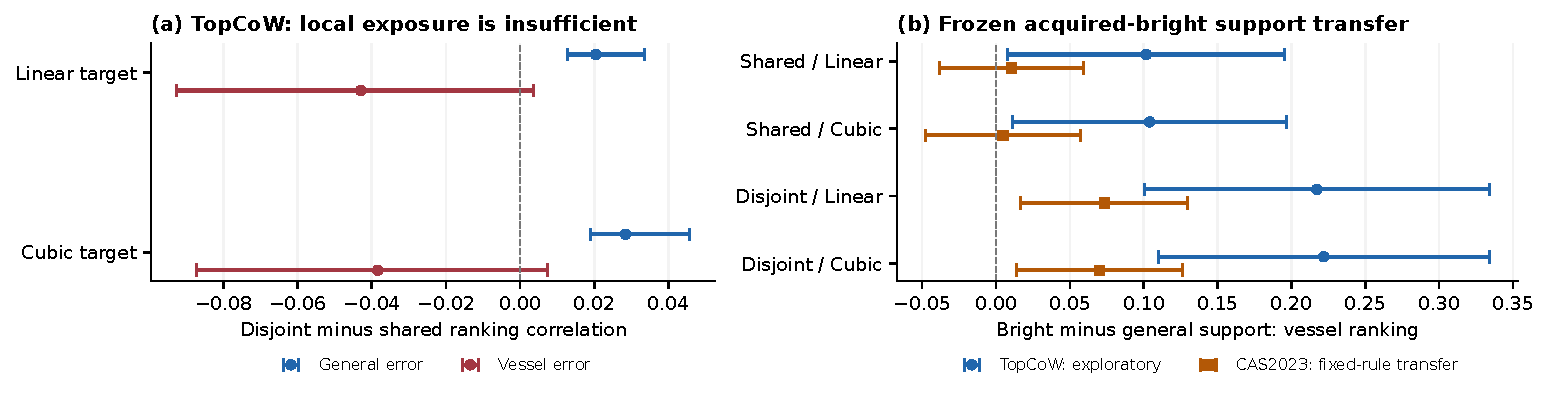
\includegraphics[width=.98\textwidth]{p14_anatomical_transfer.pdf}
\caption{Anatomical specificity with fixed analytical estimators. (a) TopCoW acquired-support scores rank general and vessel-region errors differently (pointwise intervals). (b) Bright-anchor weighting improves vessel-error ranking on TopCoW and transfers in disjoint contexts to CAS2023; intervals are simultaneous across two pairings within each cohort/context. TopCoW motivated the rule; CAS2023 received it without retuning. General-error ranking deteriorates under this weighting.}
\label{fig:topcow}
\end{figure*}

Keeping the estimator pair fixed, L$_0$--C$_2$ minus L$_0$--C$_0$ increases observable fraction by 34.5 [34.4,34.6] points; C$_0$--L$_2$ minus C$_0$--L$_0$ gives 34.5 [34.4,34.6]. Ranking changes against fixed linear/cubic error are 0.020/0.028, and against vessel-region error -0.043/-0.038 (Fig.~\ref{fig:topcow}). Vessel-risk coverage also worsens: disjoint-minus-shared normalized excess risk area is .00140 [.00028,.03211] for L and .00135 [.00026,.03120] for C. These endpoints test distinct consequences. The paired $\times4\!\rightarrow\!\times2$ control uses the same interpolation rules, eliminating factor-specific learned weights; all case-level general and vessel benefits, including negative values, are retained in the numerical record. Region-restricted intensity error is an anatomical endpoint, not segmentation or diagnostic accuracy.

\paragraph{Fixed anatomical weighting and transfer.}
After observing TopCoW's endpoint mismatch, we fix a label-free rule: retain the brightest 5\% of each acquired anchor's 1\%-foreground, then unite the nearest two anchor masks. The same TopCoW cases are exploratory development evidence. Disjoint vessel-error correlations rise from .488/.471 to .705/.693 for L/C, with changes .217 [.100,.334] and .222 [.110,.334] under two-pair simultaneous intervals.

We transfer the unchanged rule to all 100 paired CAS2023 angiograms~\cite{cas2023} (6,412 eligible planes), without fitting, label-based plane selection, or threshold search. Disjoint vessel-error correlations improve from .880/.877 to .953/.947: changes .073 [.017,.130] and .070 [.014,.126]. Shared-context changes .010/$ .005$ have simultaneous intervals crossing zero. This anatomical improvement has a cost: general-error correlations fall by .085/.084 on CAS2023 and .250/.235 on TopCoW in disjoint contexts. CAS2023 vessel-risk coverage changes favor bright weighting, but both pointwise intervals cross zero. Thus rank transfer does not establish screening utility. Labels define intensity-error endpoints, not diagnostic outcomes; CAS header provenance does not certify physical slice spacing.

\begin{table*}[t]
\caption{Reliability operating regimes; latency is measured on one representative examination per cohort}
\label{tab:operating-regime}\centering
\begin{tabular}{p{3.0cm}p{2.1cm}p{2.5cm}p{3.2cm}p{4.6cm}}
\toprule
Score&Neural calls&Measured latency&Required information&Recommended regime\\
\midrule
Adjacent-anchor MAE&0&0.69/4.00/5.24 ms&Existing sparse anchors&Default screen when no complementary reconstruction exists; strongest tested NingXia nAURC.\\
Anchor-CV&0&0.42/3.97/3.93 ms&Existing anchors with an interior holdout&Interpretable acquired-only alternate; not uniquely informative.\\
Output PC&2&1.06/10.20/11.63 ms after inference&Two stored model outputs&Useful only when outputs already exist; generation cost is not zero.\\
Architecture committee&2&0.25/2.43/0.49 s&Two trained models and outputs&Use when both architectures are already deployed; dependence remains.\\
Flip TTA&2&0.26/3.18/0.60 s&One model, same anchors, transform&Comparator for transformation variability, not a physical-independence test.\\
Measurement-disjoint&2&0.29/3.20/0.56 s&Complementary physical phase grids&Worth considering when complementary reconstructions already exist and intermediate-coverage QA matters; otherwise acquisition cost dominates.\\
\bottomrule
\end{tabular}
\end{table*}

\subsection{Failure Granularity}
Examination scores need not localize a failed plane. Historical analysis found 14 NingXia planes in the lowest PC quartile and highest error quartile; 12 were at the first generated $\times4$--$\times6$ position, suggesting shared boundary context. Controlled common blur also reduced variation while preserving error. Conversely, a strict natural fastMRI stable-wrong rule found no event. These differences motivate four failure classes: stable-wrong consensus, benign diversity, boundary-sensitive error, and global examination difficulty.

The distinction prevents an examination-level ranking from being presented as a heatmap. A high case score can prioritize review but cannot identify which slice or anatomy is wrong; a median case score can suppress an isolated catastrophic plane. Plane-localization and examination-triage endpoints must be validated separately.

\section{Discussion}
The experiments connect a familiar correlated-error limitation to a recorded imaging variable. Through-plane anchors are not generic augmentations: their physical positions determine the anatomical evidence available for the same missing plane. When contexts reuse them, errors align and a larger fraction cancels. Disjoint contexts rank intensity error and selective risk more effectively across three cohorts, while analytical factor response shows worsening consensus blindness as sampling becomes sparser.

The result separates diversity, observability, and calibration. Diversity is output distance; observability is the fraction of paired error surviving in that distance; calibration maps a score to an absolute or probabilistic statement. We study the first two. A condition can have larger raw disagreement yet poorer ranking, and no reported number supports statements such as ``this slice is correct with a given probability.''

Local exposure, examination ranking, and screening utility require separate validation. The MRA transfer makes this distinction actionable: a fixed acquired-bright score improves vessel-error ranking while losing general-error ranking, with uncertain risk-coverage benefit. A quality score should therefore specify its anatomical endpoint before evaluation.

The literature boundary is also precise. Correlated errors, systematic-error blindness, and leave-one-slice-out evaluation are not new \cite{brown2005diversity,hu2021predict,horvath2017highorder}. Recent acquisition perturbations in prostate MRI also show that variance maps can emphasize acquisition fragility while correlating only moderately with error \cite{vandervelde2026prostate}. The defensible contribution here is the target-preserving physical measurement-overlap intervention and its three-cohort endpoint, factor, geometry, failure, and selective-risk characterization.

\subsection{Comparator Semantics and Cost}
The compared scores vary different information. Disjoint phase changes physical anchor identity and requires two reconstructions plus potentially additional measurements. Maximal-shared reversal changes order but reuses evidence. The committee changes architecture while preserving acquisition. Adjacent-anchor MAE changes no output and requires zero neural calls. Predictive performance must therefore be interpreted with information availability rather than treated as an abstract leaderboard.

Representative Anchor-CV CPU scoring took 0.42/3.97/3.93 ms on fastMRI/IXI/NingXia and stored no predicted volume. Committee, flip-TTA, and disjoint pairs required two neural calls, 0.25--0.29 s / 2.43--3.20 s / 0.49--0.60 s by cohort, about 271 MiB peak allocated GPU memory, and 8.6--66.5 MiB outputs. These measurements establish computational differences only. A disjoint score can be computationally feasible yet acquisition-expensive; a zero-call input baseline can be immediately available.
The flip-TTA row is deliberately a cost comparator only: a definition-matched IXI TTA reliability output was unavailable, so no three-cohort nAURC is imputed. Output-PC times are likewise score-only and exclude generating the two prerequisite reconstructions.



\subsection{Limitations}
All phase grids are retrospective simulations from dense MRI volumes; no scanner prospectively changed sampling. NingXia has only eight independent patients. One legacy fastMRI patient overlaps train/validation, but none overlaps test; historical checkpoint-selection bias is not quantified. The full three-cohort endpoint matrix remains HAT/SwinIR and retains the historical reversal control's order confound; the clean five-architecture extension covers two brain cohorts at $\times4$, not NingXia knee. SAINT and CycleINR are adapted/internal reproductions rather than exact official implementations. The clean in-plane shared control is still an equivariance control, and identity-swap matches geometry only up to left--right reflection; neither is a prospective acquisition. The analytical factor experiment changes target availability and distance together. MRA broadens contrast and anatomical evaluation only for fixed analytical estimators; neural conclusions remain T2-specific. The densification audit is exploratory; IXI has only one recovered same-architecture pair, and factor-specific weights differ. Target-derived output masks require an acquired-only support validation before deployment. MAE/SSIM are not clinical endpoints, and there is no reader study, pathology-stratified analysis, calibrated uncertainty, or prospective adaptive acquisition.

Eligible planes are fully bracketed and exclude acquired anchors, so results need not transfer to unbracketed boundary extrapolation. The 42 endpoint rows are correlated rather than independent replications. Shared fraction is target-dependent and diagnostic, not deployable. Risk--coverage uses one frozen examination aggregation; maximum-plane or reader-task risk could reorder methods. Cross-cohort intensity calibration and prospective scanner-time utility remain unresolved.

\subsection{Evidence and Reproducibility Boundaries}
Per-plane and case-level records, source hashes, protocol amendments, and plotting scripts retain the historical and new analyses separately. TopCoW (125 cases) motivated a fixed rule subsequently evaluated on CAS2023 (100 cases); this chronology is explicit. The journal emphasizes anatomical QA and does not claim the conference paper's finite-response statistic as a new method. Shared cohorts and architecture experiments remain overlapping evidence.

\subsection{Ethics and Data Availability}
fastMRI and IXI are public deidentified resources. NingXia is an internal human MRI cohort. \textbf{[AUTHOR ACTION: insert approving/exempting institution, decision identifier, consent/waiver, and permitted-use language.] } Code, manifests, case-level derived tables, and checkpoint hashes will be released anonymously where licensing permits; raw public and internal data remain under their governing terms.

\section*{Acknowledgment}
OpenAI Codex assisted with the abstract, Sections II--VI, statistical and external-MRA scripts, and the robustness/MRA figures. The source data are pre-existing; author verification of the generated material and the final disclosure is required before submission.

\section{Conclusion}
Disagreement observes differences between reconstruction errors, not error itself. Across fastMRI, IXI, and patient-clustered NingXia, disjoint physical anchors made intensity-domain error more observable than shared-anchor output comparisons. Frozen five-architecture tests on two independent brain cohorts extend the local error-geometry effect from transformers to I3Net, an adapted SAINT-style network, and an internal CycleINR-style model; a reflection-balanced IXI control preserves it. Ranking remains cohort dependent, architectures share difficult examinations, and retrospective benefit prediction is limited by current-error coupling, intensity scale, and a degraded-model exception. The supported principle is therefore narrow: diversify influential physical evidence, validate against the intended endpoint and architecture, and never treat agreement as a correctness certificate.

\bibliographystyle{IEEEtran}
\bibliography{references}
\end{document}
